\chapter{绪论}\label{chap:introduction}
视觉目标跟踪是计算机视觉领域的一个重要研究课题,它以摄像机拍摄得到的序列图像为研究对象,其中包含与摄像机有相对运动关系的目标,以在视频的连续帧之间创建基于位置、速度、形状、纹理、色彩等有关特征的对应匹配为研究目的,建立目标在帧间的关联关系。视觉目标跟踪问题经过数十年的发展,逐步形成了以基础应用需求不同而衍生的多种特定类别目标跟踪研究。比如,针对跟踪任意运动目标的通用跟踪问题而广泛开展的模型非固定式在线视觉跟踪研究(model-free tracking,MFT);针对监控场景下广泛存在的特定运动目标(如行人、车辆等),而开展的基于特定模型检测的离线/在线多目标跟踪研究(model-based tracking,MBT);针对室内场景下类似于 Microsoft Kinect 这类 RGBD 摄像机的应用场景开展的基于深度(depth)信息的 RGBD 跟踪研究;以及针对机器人自主导航应用中的视觉里程计(visual odometry,VO)开展的基于关键特征点匹 配的相关跟踪算法研究等等。

本文主要针对模型非固定式在线视觉目标跟踪开展研究,在只有视频序列初始帧存在感兴趣目标区域标注情况下,设计跟踪算法自动完成对后续视频序列中的感兴趣目标区域的标注。模型非固定式在线视觉目标跟踪受限于缺乏目标的先验信息,且目标表观又会随着时间由于各种各样的因素发生剧烈的变化,比如噪声干扰、运动模糊、光照变化、非刚性的目标形变、视角的变化导致的目标旋转、遮挡等,因此设计鲁棒、准确的视觉目标跟踪算法面临很大的挑战。
本文基于卷积神经网络强大的表征能力,利用目标的语义信息,对视觉目标跟踪算法的表观模型构建过程进行增强;利用丰富的空间信息,对视觉目标跟踪算法的运动模型进行增强;利用丰富的时间信息,对视觉目标跟踪算法的特征提取能力进行增强;利用目标的自适应信息,对视觉目标跟踪算法的模型自适应能力进行增强;利用对抗性信息,研究视觉目标跟踪算法的鲁棒性。
本章接下来的内容,首先介绍视觉目标跟踪问题的研究背景与意义,随后阐述本文的主要内容与贡献,最后列出本文后续的章节结构。

\begin{figure}[t]
\centering
\includegraphics[width=1\textwidth]{Img/introduction/show_dataset.pdf}
\caption{本文所针对的模型非固定式在线视觉目标跟踪的典型应用场景。这些视频序列截图取自最近流行的 GOT-10k \cite{GOT-10k} 视频跟踪测试库所提供的部分视频序列。}
\end{figure}

\section{研究背景与意义}
近年来,数字媒体的快速兴起加速了人们对于视频内容的获取与传播,智慧城市的建设使得城市监控设备采集到的视频数据大规模增长。随着互联网、物联网、大数据等信息技术的兴起,高性能计算机、网络摄像机、CMOS/CCD 视觉传感器、云存储设备、高性能图形处理器(GPU)、张量处理器(TPU)等硬件设备的蓬勃发展,视频内容的成像质量、传输速度有了很大的进步,这为计算机视觉的智能化奠定了坚实的基础。视觉目标跟踪作为计算机视觉研究领域中的重要技术之一,广泛应用于智能监控、自动驾驶、军事侦察、虚拟现实、人机交互等领域,具有巨大的应用前景和商业价值。
\begin{itemize}
\item 智能监控。智能监控的目的是由计算机智能地分析摄像头所获取的图像序列,对场景内容进行理解,实现对异常行为的自动报警。智能视觉监控技术大概可以分为底层视觉和高层视觉两个部分。底层视觉主要是对场景中感兴趣目标进行检测、跟踪和识别,而高层视觉则是在底层视觉的基础上对感兴趣目标进行行为分析和理解。智能视觉监控技术可以广泛应用于公共安全监控、工业现场监控、居民小区监控、交通状态监控等各种监控场景中,能够显著提高监控效率,降低监控成本,具有广泛的研究意义和应用前景。视觉跟踪的任务就是在连续的图像序列中对运动目标进行定位,为后续行为分析提供目标轨迹和运动参数等信息。它在智能视觉监控技术中起着至关重要的作用。跟踪所提供的丰富的时间和空间信息,可以使目标检测和识别更加鲁棒;同时跟踪所提供的轨迹信息和运动参数是目标行为分析和理解的基本前提。
\item 自动驾驶。自 20 世纪 80 年代中期以来,世界各地的许多大学、研究中心、汽车公司和其他行业的公司都在研究和开发自动驾驶汽车(又称无人驾驶汽车)。自动驾驶系统的体系结构一般分为感知系统和决策系统。感知系统一般分为多个子系统,负责汽车定位、静态障碍物感知、移动障碍物检测与跟踪、道路感知、交通信号检测与识别等任务。其中,利用激光雷达(LiDAR)、摄像头、全球定位系统(GPS)、惯性测量单元(IMU)等车载传感器采集的多模态数据,对目标进行识别和跟踪,便是重要一环。跟踪其他交通参与者是自动驾驶的一项非常重要的任务。例如,由于车辆的制动距离随车辆速度成倍增加,有必要对其他交通参与者的未来运动轨迹进行准确预测,以避免交通事故的发生。因此,设计高性能的跟踪器对于自动驾驶而言十分重要。% http://www.ryxxff.com/67630.html https://arxiv.org/pdf/1704.05519.pdf
\item 军事侦察。军事侦察指为获取军事斗争所需有关战区和敌方情况而采取的措施,可以为正确进行军事指挥和获取战争胜利提供科学的依据和切实的保障。随着科学技术的发展,无人机能够较好地完成侦察、对地攻击和监视等军事任务,成为了各国普遍采用的军事侦察设备之一。而无人机之所以能够用于军事侦察,主要是由于其能够在高速运动条件下获取地面目标的动态信息,能够实现对运动目标的检测和跟踪,从而顺利完成军事侦察任务。因此,针对运动目标的跟踪技术,已经成为了军事侦察工作的核心技术手段之一。
\end{itemize}

综上所述,视觉目标跟踪技术的研究与应用对计算机视觉的发展起着重要作用。近年来,关于视觉目标跟踪的科学研究蓬勃发展。TPAMI、IJCV 等国际权威期刊,以及 CVPR、ICCV、ECCV 等计算机视觉顶级会议,都将视觉目标跟踪定义为重要研究方向。近三十年来,视觉目标跟踪领域取得了很多重要突破,产生了众多的研究成果。但是,视觉目标跟踪领域依然存在着很多理论和技术问题有待解决,特别是跟踪过程中嘈杂背景干扰、运动模糊、光照变化、目标非刚体形变、障碍物遮挡等在开放环境中遇到的复杂挑战。所以如何能够自适应、鲁棒地跟踪目标一直是广大研究人员亟需解决的问题,依然具有很高的研究价值和研究空间。

\begin{figure}
\centering
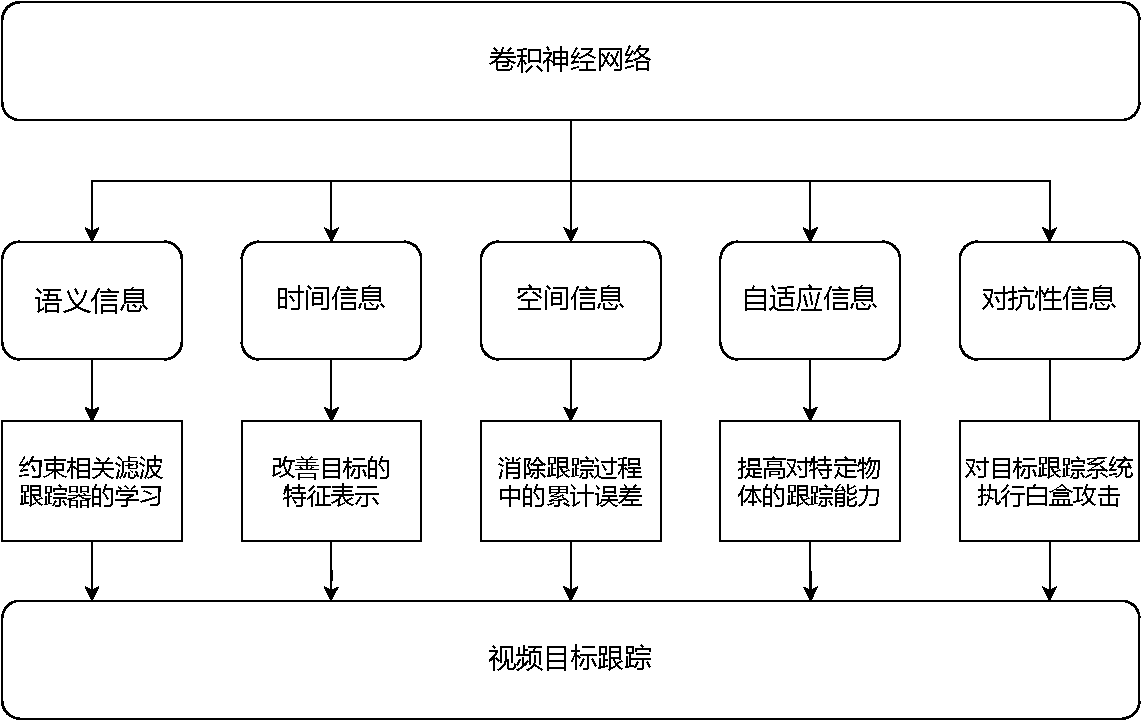
\includegraphics[width=0.75\textwidth]{Img/paper_arch.pdf}
\caption{文章组织架构。}
\end{figure}

\section{研究内容与主要贡献}
基于 MFT 的在线视觉目标跟踪的主要研究问题包括表观建模方法、运动模型设计、特征学习方法、模型更新等环节,通过对这些环节的改进,来解决在线视觉目标跟踪中的目标姿态变化、光照变化、遮挡等难点,以达到准确、鲁棒的技术指标。
本文对基于卷积神经网络的视觉目标跟踪算法做了深入研究:在表观建模方面,利用目标的语义信息,约束相关滤波跟踪器的训练过程,从而提高相关滤波器的性能。在运动模型方面,首先为孪生网络跟踪器引入更丰富的空间信息,使得跟踪器可以在整个图像平面内感知目标的位置信息;其次利用端到端训练的轨迹预测模块,预测目标在当前帧的每个空间位置上出现的可能性。在特征学习方面,为孪生网络跟踪器引入更丰富的时间信息,通过来自相邻帧的目标表观信息的聚合,使得目标表观特征更加丰富,弥补基于孪生网络的视觉目标跟踪算法局限于从单帧提取目标表观,对目标表观表示能力不足的缺点,从而提高跟踪的效果,实现鲁棒的跟踪。在模型更新方面,为孪生网络跟踪器引入自适应信息,通过对模板图像的像素进行轻微扰动,改善孪生网络跟踪器对于特定目标的跟踪性能。最后,为了研究视觉目标跟踪算法相对于对抗样本的鲁棒性,将对抗性信息应用到孪生网络跟踪器中,为基于孪生网络的视觉目标跟踪算法生成视频无关的通用扰动,从而使得跟踪器做出错误的行为。具体地,本论文的研究内容主要包含以下部分:
\begin{itemize}
\item \textbf{提出了一种语义信息引导的视觉目标跟踪算法}。
首先,本文利用一个深层卷积神经网络,为目标生成实例级别的语义分割掩码,用于约束相关滤波器的学习,以提高跟踪的鲁棒性。其次,针对离线训练的语义分割结果和在线学习的相关滤波结果具有互补性这一特点,进一步提出了一种自校正机制,来缓解相关滤波跟踪器的漂移问题。本文在多个具有挑战性的视觉目标跟踪标准库上验证了这些创新点在视觉目标跟踪任务中的有效性。
\item \textbf{提出了一种空间信息增强的视觉目标跟踪算法}。
本文从基于局部感知机制的孪生网络跟踪器鲁棒性不足问题出发,利用全局感知机制在整个图像平面上感知物体的位置信息,来弥补孪生网络跟踪算法容易造成跟踪结果的累积误差导致跟踪漂移,且在长期跟踪任务上表现不佳的问题,实现鲁棒的跟踪。本文采用了两阶段的目标跟踪框架,利用深层卷积神经网络进行特征提取,因此目标特征具有较强的判别性。此外,本文还添加了基于卷积神经网络的轨迹预测模块,该模块利用目标的历史运动信息来减轻近似物体的干扰。
本文在流行的视觉目标跟踪标准库上进行了算法的对比实验、成分分析实验以及定性评估实验,从而验证算法改进的有效性。
\item \textbf{提出了一种时间信息增强的视觉目标跟踪算法}。
首先,将时间聚合模块应用到基于孪生网络的视觉目标跟踪算法中,通过聚合来自相邻帧的时间信息来改善每帧的特征,从而可以使孪生网络跟踪器处理由运动模糊等原因造成的较差的目标表观。其次,本文在基于孪生网络的视觉目标跟踪算法中整合了对抗性 Dropout 模块,以端到端的方式学习具有判别性的目标特征。本文在多个视觉目标跟踪标准库上验证了算法的有效性,并在准确性和鲁棒性上取得了较好的结果。
\item \textbf{提出了一种自适应信息增强的视觉目标跟踪算法}。本文通过简单地在孪生网络中操纵模板图像的像素,来处理视觉目标跟踪中具有挑战性的模型自适应任务。对模板图像像素进行稍加修改,即可改善离线训练的孪生网络对于不包含在训练集中目标的跟踪结果。本文采用流行的对抗样本生成方法执行模板像素的操纵,以进行模型自适应。与大多数模板更新方法(旨在融合先前帧的目标特征)不同,本文专注于在第一帧中使用目标的真实标注信息进行模型的初始自适应。本文的模型自适应方法是即插即用的,不会改变其基线跟踪器的总体架构。本文在目前比较流行的视觉目标跟踪标准库上验证了所提算法的有效性。
\item \textbf{研究了对抗性信息在视觉目标跟踪算法中的应用}。
本文提出了一种通用的对抗样本,可以对基于孪生网络的视觉目标跟踪算法进行对抗性攻击。具体来说,通过向模板图像添加通用的半透明的微小扰动,并将虚假目标(一个小的对抗图像补丁)添加到搜索图像中,使得跟踪器预测虚假目标,而非真实目标的位置和大小。所提出的对抗性扰动信息通过离线的大规模视觉目标跟踪数据集训练得到,可在占用极少计算资源的情况下对任意视频进行有效攻击。在多个视觉目标跟踪标准库上的实验结果表明,该方法能够有效地欺骗孪生跟踪器。
\end{itemize}

\section{后续章节安排}
\begin{itemize}
\item 第二章:基于深度学习的视觉目标跟踪算法综述。基于深度学习,尤其是基于卷积神经网络的视觉目标跟踪算法既是当前视觉目标跟踪领域的研究热点,也是本文的研究重点。本章将基于深度学习的跟踪器划分为以下几种类别:基于深度特征的相关滤波跟踪器、基于生成对抗网络的跟踪器、基于图卷积网络的跟踪器、基于循环神经网络的跟踪器、基于脉冲神经网络的跟踪器、基于孪生网络的跟踪器、基于强化学习的跟踪器、基于元学习的跟踪器、基于无监督学习的跟踪器、基于注意力机制的跟踪器和基于串并联或级联结构的跟踪器。
\item 第三章:本章提出了语义信息引导的视觉目标跟踪算法。本章从解决基于相关滤波的在线视觉目标跟踪器缺乏高层语义信息指导这一问题出发,结合当前主流卷积神经网络提取图像语义信息方面的研究进展,提出了实例引导的相关滤波器。本章介绍了图像分割网络的整体损失函数和网络架构设计,用于约束基于相关滤波的表观建模过程。然后分别阐述了网络的训练步骤以及在线跟踪策略。最后,本章对网络的各个组成部分进行了实验分析,验证了它们的有效性,并在多个视频跟踪标准评测库上测试了算法的整体跟踪性能。
\item 第四章:本章提出了空间信息增强的视觉目标跟踪算法。首先,本章分析了当前基于孪生网络的在线视觉目标跟踪算法采用的局部搜索机制的不足。然后介绍了本章利用全局感知机制以增强空间信息的实现方案。在全局感知机制的基础上,本章进一步引入了基于卷积神经网络的轨迹预测模块。本章在多个视频跟踪标准库上验证了全局感知机制和轨迹预测模块的有效性以及整体跟踪性能。
\item 第五章:本章提出了时间信息增强的视觉目标跟踪算法。首先,本章分析了流行的基于孪生网络的在线视觉目标跟踪算法在利用时间信息方面的不足。然后介绍了如何在卷积神经网络中融合时间信息,从而丰富目标的特征表示。最后,本章引入了对抗性 Dropout 模块,进一步提高了目标特征的鲁棒性,并在视觉目标跟踪标准评测库上验证了算法的有效性。
\item 第六章:本章提出了自适应信息增强的视觉目标跟踪算法。本章从解决基于孪生网络的在线视觉跟踪中的离线训练模型无法处理跟踪目标的丰富表观问题出发,结合当前主流视觉目标跟踪算法在解决模型自适应问题方面的研究进展,提出了自适应信息增强的视觉目标跟踪算法。本章介绍了训练自适应信息的整体损失函数以及网络架构设计,用于获取目标的自适应信息。然后阐述了网络训练的步骤。最后,本章对网络的各个组成部分进行了实验分析,验证了它们的有效性,并在多个视频跟踪标准评测库上测试了算法的整体跟踪性能。
\item 第七章:本章提出了对抗性信息在视觉目标跟踪算法中的应用。首先,本章分析了当前基于孪生网络的在线视频跟踪算法容易受到对抗性扰动信息攻击的现象,以及现有针对孪生网络的攻击算法在性能和效率上的不足。然后介绍了利用视频无关的通用对抗性信息对孪生网络跟踪器进行对抗攻击的实现方案。本章在多个视频跟踪标准评测库上验证了本章所提出的对抗攻击方法的有效性。最后,本章将所设计的对抗性扰动应用于不同的网络结构以及不同的跟踪框架,验证了所提出方法的可迁移性。
\item 第八章:对本文研究内容进行客观全面的总结,并对个人下一步的研究计划进行了分析和讨论。
\end{itemize}